\chapter{Elementary Geometry: From Measurement and Construction to Proof}

In the first two chapters, symbols and equations compressed many concrete problems into models we could carry from one situation to another. Most belonged to the world of quantities: prices, speeds, and times. In this chapter we enter a different world---the world of shapes. You will see that humanity's earliest geometrical knowledge arose from practical needs: surveying land, building houses, and observing the stars. Yet geometry's most remarkable achievement was eventually to escape the limitations of rulers and ropes and become a subject whose conclusions could be guaranteed by reasoning alone. This was the first appearance of proof in the history of mathematics, and the first appearance of a theme that will echo throughout this book.

\section{A Pyramid in the Shadows}

About twenty-six hundred years ago, a traveller arrived in Egypt. Standing before an enormous pyramid, he asked a question that left the local priests bewildered: how tall is it?

Direct measurement was impossible. The pyramid's sides were sloping walls of stone. No ladder could reach its tip, and no rope could be lowered from the top---the tools of the day could not reach a summit more than a hundred metres high. The traveller did not climb the pyramid. He asked only for a wooden pole, a length of rope, and a sunny day.

He planted the pole vertically in the ground and waited for the sunlight. The pole cast a shadow on the ground, and the pyramid cast a great shadow across the sand. He measured three quantities: the pole's height, the length of its shadow, and the length of the pyramid's shadow (from the edge of its base to the shadow's tip, plus half the length of the base, because the centre of the base lies directly below the summit). Then a simple proportion gave him the pyramid's height, reportedly with very little error.

The traveller was Thales of ancient Greece. Legend says that the priests were astonished, but do not rush to admire him just yet. A real mathematical question lies inside this story, and it is where our chapter begins.

\section{What Justifies It, and What Does Not}

Why was Thales's method correct? His intuition was probably this: at the same moment, sunlight falls at the same angle, so the small triangle formed by the pole and its shadow and the large triangle formed by the pyramid and its shadow are enlarged versions of the same shape. When shapes are the same, corresponding sides have the same ratio, so

\[
\frac{\text{pyramid height}}{\text{pole height}}=\frac{\text{pyramid shadow}}{\text{pole shadow}}.
\]

Knowing three of these four quantities lets us calculate the fourth. For instance, if the pole is $2$ metres tall, its shadow is $3$ metres long, and the pyramid's shadow (measured from its centre) is $180$ metres long, then the pyramid is $2\times 180\div 3=120$ metres tall.

This reasoning sounds natural. But pause and ask one more question, as a mathematician would: why does ``the same shape'' imply ``proportional corresponding sides''? Measure a hundred triangles and it will seem true every time. Yet a gulf separates ``the measurements agree'' from ``it must be true.''

Consider an easy trap. Draw a triangle, measure its three interior angles with a protractor, and add them. What do you get? Probably not exactly $180^\circ$: perhaps $179^\circ$ or $181^\circ$. Draw another, measure again, and you are still a little off. You might say that the protractor is inaccurate and that the sum should theoretically be $180^\circ$. Good---but where did that ``theoretically'' come from? You have not measured every triangle in the world, or even a hundred million. Even if a hundred million all gave something close to $180^\circ$, what about the next one? A triangle with sides a light-year long? One too small to see?

This is the division of labour between measurement and proof. Measurement is a tremendous achievement: it helps us discover patterns and make conjectures, and engineers use it to build real bridges. But measurements always carry errors and can check only finitely many examples. Geometry is full of conclusions about infinitely many cases. ``The interior angles of every triangle sum to $180^\circ$'' refers to every triangle, whatever its size or proportions. A ruler cannot handle ``every''; reasoning can.

This also explains why the ancient Egyptians could survey land and build pyramids without leaving behind a concept of the theorem, whereas the ancient Greeks turned geometry into a science of proof. Measurement tells us approximately what is true; proof tells us why it must be true. Our goal in this chapter is to travel from ``approximately'' to ``necessarily.''

\section{From ``They Look the Same'' to Definitions}

To replace measurement with reasoning, we must first turn vague everyday words into precise definitions. You may think you understand ``point,'' ``line,'' and ``angle,'' but try explaining them clearly to someone who has never seen them. It is harder than it sounds.

The ancient Greeks took a somewhat surprising approach: they admitted that the most basic concepts could not truly be defined, only stipulated. A point is a position without size, a line has length without width, and a straight line can extend indefinitely in both directions. These statements tell us less about what a point ``is'' than about the rules it obeys. For example, we agree that exactly one straight line passes through two distinct points, and that a line segment is the shortest path between two points. Such agreements are called axioms. They are the starting points of reasoning, just as the moves of the horse and elephant must be agreed upon before a game of Chinese chess.

With points and lines, we can create our first real object of study: join three line segments end to end to enclose a figure, and we have a triangle. Triangles are the atoms of geometry. Every polygon can be divided into triangles, so understanding triangles comes close to understanding all of plane geometry.

Next come two crucial concepts, both obtained by unpacking the everyday word ``same.''

\begin{dingyi}[Congruence]
Two figures are \textbf{congruent} if translations, rotations, and reflections can make them coincide exactly. Congruent triangles have equal corresponding sides and equal corresponding angles. We write $\triangle ABC \cong \triangle DEF$.
\end{dingyi}

\begin{dingyi}[Similarity]
Two figures are \textbf{similar} if they have the same shape, though their sizes may differ. Two triangles are similar if and only if their corresponding angles are equal; their corresponding side lengths then share a common ratio, called the similarity ratio.
\end{dingyi}

Congruence means ``coinciding exactly''; similarity means ``different scalings of the same shape.'' Thales used similarity to measure the pyramid: the pole triangle and pyramid triangle are similar, and their similarity ratio is the ratio of the shadow lengths.

\begin{shuyu}{Congruence}
Intuition: figures cut from the same mould, fitting perfectly on top of one another after shifting, turning, or flipping.
Formal definition: two figures that coincide exactly after translations, rotations, and reflections.
Example: two identical triangular pieces of paper made with a photocopier are congruent.
\end{shuyu}

\begin{shuyu}{Similarity}
Intuition: a photograph and its enlargement have the same shape but different sizes.
Formal definition: two figures whose corresponding angles are equal and whose corresponding sides share a common ratio.
Example: a triangular plot on a map is similar to the real triangular plot; the similarity ratio is the map's scale.
\end{shuyu}

Definitions tell us what ``the same'' means, but not how to recognize it. We often cannot place two triangles on top of each other---you cannot move a pyramid. Fortunately, mathematicians discovered that checking triangle congruence does not require comparing all six quantities (three sides and three angles). The right three are enough:

\begin{itemize}
\item Three corresponding sides are equal (side--side--side).
\item Two corresponding sides and their included angle are equal (side--angle--side).
\item Two corresponding angles and their included side are equal (angle--side--angle).
\end{itemize}

These criteria contain claims that can be proved. For side--angle--side, for example, the intuition is that fixing the lengths of two sides and their included angle determines the third side uniquely; the triangle has no room to change shape. Similarity has its own economical criterion: two equal corresponding angles suffice. Since the interior angle sum of a triangle is fixed (as we will prove shortly), fixing two angles fixes the third, and the shape is locked in place.

\begin{fanli}
``If two corresponding sides and the angle opposite one of them are equal, the triangles are congruent.'' This sounds much like the earlier criteria, but it is false. Fix side $AB$, side $AC$, and angle $B$ (notice that $B$ is not the angle included between $AB$ and $AC$). Point $C$ must lie on the ray from $B$ making the prescribed angle with $BA$, while also satisfying the prescribed length of $AC$. In other words, it is an intersection of that ray with an arc centred at $A$ and having the given radius. The arc may meet the ray at \textbf{two} different points, producing one broad triangle and one narrow triangle that satisfy the same conditions but are not congruent. This trap reminds us that every word in a criterion matters: replace ``included angle'' with ``opposite angle'' and the conclusion collapses. It is also a natural place for proof by cases to enter: when the same conditions can produce two figures, each possibility must be checked separately.
\end{fanli}

Before continuing, let us supply the proof we owe. It is also our first important example of a geometrical proof technique: adding an auxiliary line.

\begin{dingli}[The Interior Angle Sum of a Triangle]
The three interior angles of any triangle sum to $180^\circ$.
\end{dingli}

\begin{center}
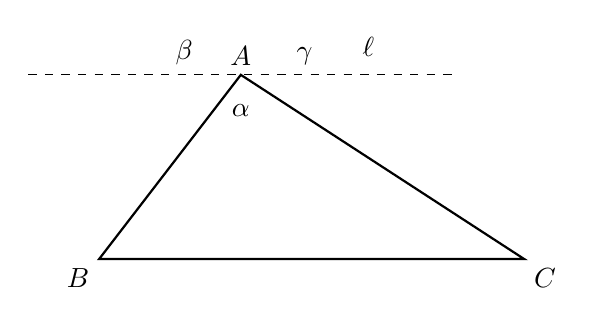
\begin{tikzpicture}[scale=0.9]
\draw[thick] (0,0) -- (6,0) -- (2,2.6) -- cycle;
\draw[dashed] (-1,2.6) -- (5,2.6);
\node[below left] at (0,0) {$B$};
\node[below right] at (6,0) {$C$};
\node[above] at (2,2.6) {$A$};
\node at (3.8,3.0) {$\ell$};
\node[above] at (1.2,2.6) {$\beta$};
\node[above] at (2.9,2.6) {$\gamma$};
\node at (2,2.1) {$\alpha$};
\end{tikzpicture}
\end{center}

\begin{proof}
Let the triangle be $\triangle ABC$. Through vertex $A$, draw a line $\ell$ parallel to side $BC$ (the dashed line in the figure). This line was not in the original figure: we \textbf{added} it to help our reasoning, so it is called an auxiliary line.

Side $AB$ crosses both parallel lines $\ell$ and $BC$, so the angle $\beta$ formed by $AB$ and $\ell$ to the left of $A$ equals angle $B$ (alternate interior angles are equal). Similarly, the angle $\gamma$ formed by $AC$ and $\ell$ to the right of $A$ equals angle $C$. At $A$, however, $\beta$, angle $A$ itself (labelled $\alpha$), and $\gamma$ fit together into a straight angle, or $180^\circ$. Therefore
\[
\angle A+\angle B+\angle C=180^\circ.
\]
Notice that this argument measures no angle. It works for every triangle, whatever its side lengths.
\end{proof}

The move worth savouring is ``draw a parallel line.'' It was not originally there; we invited it in to help. Once it arrives, angles $B$ and $C$ are carried over beside $A$. The three angles stand shoulder to shoulder along a straight line, and the conclusion emerges. Auxiliary lines are among the most creative parts of geometrical proof: there is no fixed recipe, only an understanding of the figure and a little luck. You will see more of their performances later.

\section{One Theorem, Two Reasons}

Now for this chapter's leading character. Right triangles are a special family: one angle is exactly $90^\circ$. The two sides enclosing the right angle are called the legs; the longest side, opposite the right angle, is the hypotenuse. They satisfy what may be the world's most famous theorem.

\begin{dingli}[The Pythagorean Theorem]
The sum of the squares of the legs of a right triangle equals the square of its hypotenuse. If the legs have lengths $a$ and $b$, and the hypotenuse has length $c$, then
\[
a^2+b^2=c^2.
\]
\end{dingli}

Try a few numbers. $3$, $4$, $5$: $9+16=25$, correct. $5$, $12$, $13$: $25+144=169$, correct. The ancient Egyptians used $3$, $4$, $5$ to make right angles with ropes: mark twelve equally spaced knots on a rope and form a triangle with sides of $3$, $4$, and $5$ intervals, and its largest angle is a right angle. But the same issue returns: checking ten thousand triples is not a proof. Here are two entirely different proofs---one conclusion, two different reasons. That itself is an important mathematical fact: a theorem belongs to its conclusion, not exclusively to any particular proof; another proof gives another way to understand it.

\textbf{Proof 1: Rearranging Areas.}

\begin{center}
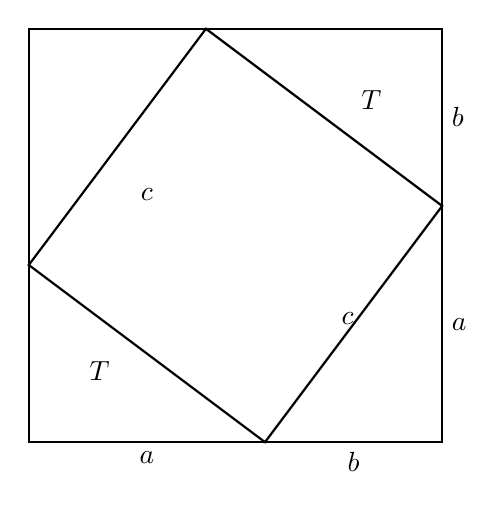
\begin{tikzpicture}[scale=0.75]
\draw[thick] (0,0) -- (7,0) -- (7,7) -- (0,7) -- cycle;
\draw[thick] (4,0) -- (7,4) -- (3,7) -- (0,3) -- cycle;
\node at (2,4.2) {$c$};
\node at (5.4,2.1) {$c$};
\node[below] at (2,0) {$a$};
\node[below] at (5.5,0) {$b$};
\node[right] at (7,2) {$a$};
\node[right] at (7,5.5) {$b$};
\node at (1.2,1.2) {$T$};
\node at (5.8,5.8) {$T$};
\end{tikzpicture}
\end{center}

\begin{proof}
Take four congruent right triangles with legs $a$ and $b$ and hypotenuse $c$. Arrange them inside a large square of side $a+b$, one triangle in each corner with its hypotenuse facing inward. The four hypotenuses enclose a central quadrilateral.

First confirm that the central region really is a square. All four sides have length $c$, so we need only check one angle. At a joining point along the bottom side of the large square, an acute angle $\alpha$ of one triangle, an acute angle $\beta$ of another, and an angle of the central quadrilateral form a straight angle of $180^\circ$. But $\alpha+\beta=90^\circ$, since they are the two acute angles of the same right triangle. The central angle is therefore $90^\circ$. A rhombus with four equal sides and one right angle is a square, with area $c^2$.

Now calculate the area of the same large square in two ways. Directly it is $(a+b)^2$. By pieces it is the four triangles plus the central square. Each triangle has area $\frac{1}{2}ab$, so
\[
(a+b)^2=4\times\frac{1}{2}ab+c^2=2ab+c^2.
\]
Expanding the left side gives $a^2+2ab+b^2=2ab+c^2$. Subtract $2ab$ from both sides to obtain $a^2+b^2=c^2$.
\end{proof}

What is the heart of this proof? \textbf{Area does not change when pieces are cut apart and rearranged.} The figure changes shape, but its area stays fixed: area is an invariant of cutting and rearrangement. Finding a quantity that remains unchanged amid change is often the key to a proof. This idea will return repeatedly.

\textbf{Proof 2: Using Similarity.}

\begin{proof}
Let $\triangle ABC$ be a right triangle with its right angle at $C$ and hypotenuse $AB$. Draw the perpendicular from $C$ to $AB$, meeting it at $D$---another auxiliary line. It splits the original triangle into two smaller triangles, $\triangle ACD$ and $\triangle CBD$.

Compare $\triangle ACD$ with the original $\triangle ABC$: they share angle $A$, and each has a right angle ($ADC$ and $ACB$). Two corresponding angles are equal, so the triangles are similar. Likewise, $\triangle CBD$ is similar to $\triangle ABC$. Write down the ratios of corresponding sides. Set $AB=c$, $AC=b$, $BC=a$, and write $AD$ as $x$ and $BD$ as $y$, noting that $x+y=c$. From $\triangle ACD \sim \triangle ABC$ (hypotenuse corresponding to hypotenuse, and leg $AC$ to leg $AD$),
\[
\frac{AC}{AB}=\frac{AD}{AC},\quad\text{that is, } b^2=cx.
\]
Similarly, $\triangle CBD \sim \triangle ABC$ gives $a^2=cy$. Add the two equations:
\[
a^2+b^2=cx+cy=c(x+y)=c^2.
\]
Here we used the basic property that corresponding sides of similar triangles are proportional. Its rigorous proof needs more preparation, so in this chapter we accept it as a tool, just as we agree on the rules before playing a game.
\end{proof}

Compare the flavour of these two reasons. The first makes the theorem a story about area: $a^2$, $b^2$, and $c^2$ are no longer abstract squares of numbers but three tangible square regions that we could cut out and weigh. The theorem says that the two smaller squares can fit together to make the large square on the hypotenuse. The second makes it a story about shape: a right triangle contains two smaller versions of itself, and that self-similar structure forces the equality. Neither proof measures a length, and both work for every right triangle.

Incidentally, there may be hundreds of proofs of this theorem: some use trapezoid areas, others circles, and still others pure algebraic completion of squares or another arrangement of the hypotenuse diagram (see the exercises). Mathematicians still occasionally publish new proofs, because each new reason may illuminate a new aspect of the theorem and prove useful elsewhere.

\section{Invariants, Cases, and Circles}

Our two proofs of the Pythagorean theorem used two general weapons: invariants and auxiliary lines. This section puts a third on the table and then sends them all to work on circles.

\textbf{Proof by cases} means something simple: when a statement's conditions allow several different possibilities, separate them completely and solve each one. In the earlier side--side--angle counterexample, an arc and a ray may intersect at zero, one, or two points. These cases yield nonexistence, uniqueness, or two solutions; without separating them, we cannot describe the outcome clearly. Another example is deciding whether three segments can form a triangle. We need only the following fact, which follows directly from ``a segment is the shortest path between two points.''

\begin{tuilun}[The Triangle Inequality]
The sum of any two sides of a triangle is greater than the third side. Conversely, if the sum of the two shorter of three segments exceeds the longest, they can form a triangle.
\end{tuilun}

Notice that this corollary already embodies the idea of cases: instead of checking all three pairs, we need check only the crucial case of whether the two shortest sides together exceed the longest.

An \textbf{invariant} reverses the question: while the figure changes, what stays fixed? Area stays fixed under cutting and rearrangement; angles and shape stay fixed under enlargement and reduction (the whole point of similarity). Circles give an even more beautiful example.

Define a circle as all points at a fixed distance (the radius $r$) from a fixed point (the centre), and consider its circumference. Measure a few circles with string---a coin, a cup rim, a round table---and you will find that circumference divided by diameter is always about $3.14$. Again, measurement suggests a conjecture. Why must it hold? Because any two circles are similar: enlarge a circle about any point and it remains a circle. Ratios of corresponding lengths in similar figures are fixed, so the ratio of circumference to diameter is the same for every circle. This number is $\pi$. It is irrational, with a decimal expansion that never ends; $3.14$ and $3.14159$ are only approximations. Ancient mathematicians found an ingenious way to approach it: inscribe regular polygons inside a circle. As the number of sides grows, their perimeters approach the circumference. Bounds from regular $96$-gons place $\pi$ between $3.1410$ and $3.1427$---an achievement of Archimedes' era, and an early victory of approximating the infinite with the finite. We will return to this picture when discussing limits in Chapter 11.

\begin{shuyu}{Invariant}
Intuition: while everything else changes, it refuses to change, making it a useful yardstick and witness.
Formal definition: a quantity or property preserved by a specified operation or transformation.
Example: area is unchanged when paper is cut and rearranged, so calculating the same area in two arrangements can prove the Pythagorean theorem.
\end{shuyu}

Area itself deserves a definition. Defining it rigorously is not easy (integration in Chapter 12 will truly address it), but at the middle-school level we can agree that a square of side $1$ has area $1$, and that area is additive and unchanged by cutting and rearrangement. It follows that a rectangle has area length times width; a parallelogram has area base times height (move a right triangle from one side to the other to make a rectangle); a triangle has half the product of base and height (two congruent triangles form a parallelogram); and a circle has area $\pi r^2$ (cut it into many small sectors and alternate them to approximate a rectangle of length half the circumference, $\pi r$, and width $r$---another preview of approximation). Behind every formula stands a rearrangement, not a measurement.

\begin{toolbox}
The new tools in this chapter:
\begin{itemize}
\item \textbf{Axioms and definitions}: reasoning begins with rules to obey; distinguish congruence and similarity within the everyday idea of sameness.
\item \textbf{Congruence and similarity criteria}: the right two or three conditions determine the shape without overlaying the figures.
\item \textbf{Auxiliary lines}: invite extra lines to help; parallel lines carry angles, and perpendicular lines create right angles and similarity.
\item \textbf{Proof by cases}: when conditions allow several possibilities, separate them completely and handle each; overlooking cases causes the side--side--angle trap.
\item \textbf{Invariants}: area under rearrangement, angles under scaling, and $\pi$ shared by all circles---a fixed quantity gives us a grip on change.
\item \textbf{Measurement and proof}: measurement discovers conjectures and supplies examples; proof guarantees all cases.
\end{itemize}
\end{toolbox}

\section{Another Perspective: Triangulation and the Stars}

Geometry's most spectacular applications rest on its most abstract conclusions. The ancient Greeks wanted to know the distances to the Moon and Sun. They had no rockets, only similar triangles and angles.

Their method is still used today and is called triangulation. To measure an inaccessible point $C$, first choose two points $A$ and $B$ and measure the baseline $AB$. Then measure the angles that the sight lines $AC$ and $BC$ make with that baseline. Two angles and the included side completely determine $\triangle ABC$. Although $C$ may be far away, the triangle's shape is fixed. Draw a scaled-down copy, or calculate using similarity and proportions, and out come $AC$ and $BC$. A surveyor measuring a tower across a river, a mapping team charting a country, and astronomers observing the Moon from two stations on Earth all use the same method. Later, people even tried using Earth itself as a baseline to measure planetary distances.

Notice the premise: we trust statements such as ``two angles and their included side uniquely determine a triangle'' and ``corresponding sides of similar triangles are proportional'' to hold equally for triangles on the ground and triangles as large as the distance to the Moon. If these were merely observations from measuring many small triangles, extending them to astronomical scales would be a huge gamble. Because they are theorems, engineers and astronomers dare to stake their work and lives on them. That is the practical value of proof: it gives knowledge a licence to operate at any scale.

\begin{lianjie}
Looking back: Chapter 1's symbols and proportions became similarity ratios and area formulas here; Chapter 2's equations let us solve for unknown sides in $a^2+b^2=c^2$. Looking ahead: throughout this chapter we drew on an unnamed plane, where points had positions but no addresses. Next chapter we will give each point an identity card bearing two numbers---its coordinates. Lines and circles will become equations; geometry problems can be calculated algebraically, and algebraic expressions can be drawn as shapes. You are about to see this chapter's theorems, especially the Pythagorean theorem, become one of the busiest formulas in the coordinate world: the distance formula.
\end{lianjie}

\section{Try It Yourself}

\begin{shiyan}
\textbf{Experiment 1: A Right Angle from Knots.} Find a soft rope and mark $12$ equally spaced knots with a marker. Form a triangle whose sides contain $3$, $4$, and $5$ intervals, pull it taut, and compare its largest angle with the right angle of a set square. Then try $5$, $12$, and $13$ intervals (requiring $30$ intervals altogether). Think: why do you believe the taut rope produces a right angle? Is that a conclusion from measurement or from a theorem?

\textbf{Experiment 2: A Paper Proof of Pythagoras.} Draw a right triangle on squared paper with legs of $3$ and $4$ squares, then make three copies (or draw three congruent triangles). Arrange the four triangles inside a $7\times7$ square as in Proof 1, and count the area of the empty square in the middle. $49-4\times6=25$, exactly $5\times5$. Repeat with different legs, such as $2$ and $5$ squares, and check whether the central area is $2^2+5^2=29$ squares.

\textbf{Experiment 3: Approaching $\pi$.} Use a compass to draw a circle of radius $5$ centimetres. With a ruler, construct an inscribed regular hexagon and then a regular dodecagon, bisecting each arc. Measure the polygon perimeters, divide by the diameter of $10$ centimetres, and record how the results approach $3.14$. Remember: however carefully you measure, this remains measurement; exact properties of $\pi$ require reasoning.
\end{shiyan}

\section*{Questions to Think About}

\textbf{Observation}
\begin{sikao}
\item Draw three triangles with very different shapes: one tall and thin, one broad and flat, and one nearly equilateral. Measure and add each one's interior angles, recording each error. Are the errors sometimes positive and sometimes negative, or always in one direction? Hint: consider the smallest divisions of your protractor and your reading habits. Where does the error come from?
\item Measure the shadow of the same vertical flagpole at different times of day. Does ``pole height divided by shadow length'' change? Hint: when would this ratio be the same? What changes, and what is invariant?
\end{sikao}

\textbf{Proof}
\begin{sikao}
\item There is another arrangement of the hypotenuse diagram: put four congruent right triangles with legs $a$ and $b$, where $a<b$, inside a large square of side $c$, with their hypotenuses along the square's four sides and a small empty square in the middle. Hint: the small square has side $b-a$. Calculate the large square's area in two ways.
\item Prove that the two base angles of an isosceles triangle are equal. Hint: bisect the vertex angle (or draw the altitude to the base), dividing the triangle into two pieces, and use a congruence criterion to show that the pieces are congruent.
\end{sikao}

\textbf{Challenge}
\begin{sikao}
\item Prove that if one side of a triangle inscribed in a circle is a diameter, the angle opposite it is a right angle. Hint: join the centre to that angle's vertex. The circle is divided into two isosceles triangles; give their four base angles two names and use the angle sum.
\item More than two thousand years ago, someone calculated Earth's circumference using these facts: at noon on the summer solstice, sunlight reached the bottom of a well in one city, producing no shadow; at the same time in a city to the north, a pole's shadow indicated an angular deviation of about one-fiftieth of a full turn; and the distance between the cities was known. Hint: treat sunlight as parallel lines. What figure do the two cities and Earth's centre form? Which central angle equals the shadow's angular deviation? What assumptions do you need, and which is only approximately true?
\end{sikao}

\begin{pandeng}
More than two thousand years ago, this chapter's picture was organized systematically in a book called the Elements: from five axioms it derived hundreds of theorems. This axiomatic style remains a standard currency of mathematics. Further ahead you will encounter Euclid's fifth postulate (the parallel postulate) and non-Euclidean geometry---replace it, and triangle angles no longer sum to $180^\circ$; projective geometry, the study of perspective and shadows themselves; trigonometry, which distils similar triangles into the sine and cosine functions; analytic geometry, next chapter's starting point, which tames curves with equations; and modern automated geometry and computer-assisted proof, where machines too can act as geometers.
\end{pandeng}

\section*{The Door to the Next Chapter}

This chapter taught us to prove things on a blank sheet: add auxiliary lines, find congruence, use similarity, and identify invariants. But you may have noticed a quiet inconvenience---points on the page have no names. We say ``the foot of the perpendicular on the hypotenuse'' or ``three centimetres to the right of the centre,'' relying on gestures and descriptions. What if a geometry problem has a hundred points and twenty curves? What if you want a computer with no eyes to draw figures or test conjectures? It cannot understand ``the point on the left.'' It understands numbers.

So a question almost childlike in its simplicity arises: can every point in the plane have a name made of numbers? If so, the distance between two points becomes an arithmetic problem, lines and circles become equations, and every theorem in this chapter gains a new language. Next chapter we will build that bridge, starting from the Pythagorean theorem and fitting the plane with coordinates.
